\chapter{Open Computing Language}
The focus of this thesis is to adapt the well reviewed, functional algorithm into the context of GPU programming practice with the help of Open Computing Language (OpenCL). Normal software often runs on processors, which could provide a very high clock speed but a rather small number of threads, hence a graphic card could perform much better at certain tasks. The design of a graphic card allows it to be very efficient at graphic manipulation, image processing etc.. In the following section of the thesis the design and specification of a graphic card is introduced to provide an insightful overview of how it works and why it is important to have the right configuration for the best possible performance.  
\section{Graphic Processing Unit}
Graphic processing units (GPUs), which is defined as "a specialized electronic circuit designed to rapidly manipulate and alter memory to accelerate the creation of images in a frame buffer intended for output to a display device", are widely used in modern devices such as computers, embedded systems and gaming consoles. GPUs have a highly parallel architecture and a very high number of cores, which make them very efficient on tasks that can be highly parallelized, such as matrix calculation, image processing etc..  For example, the latest Intel central processing unit (CPU) Core i9 has only 6 cores and 12 threads while the latest GPU by NVIDIA, the GTX 1080, has 2560 Cores, which is around 400 times the number of cores of the i9.

Although each core of a CPU could show a superior clock speed, which is 2-3x faster than a GPU core depending on type and generation, a GPU has far more cores to work with. For tasks that could be divided into smaller subtasks and executed in a parallel way, using GPU often shows a much better result.

In our thesis, the transformation of points with transformation matrices is a task that is very independent and repeating. Therefore running a shifting algorithm with the help of a CPU is very disadvantageous, mainly due to two reasons:

\begin{itemize}
	\item CPUs in single CPU systems are normally preoccupied by another process in an operating system. Depending on the cores and threads available it is not possible to fully parallelize all combinations even with server oriented processors. Therefore the combinations, which could be several hundreds, would be executed one after each other.

	\item GPUs, on the other hand, can be used as a dedicated unit for the task only. It is even possible to use more than one GPU at a time, in case the number of threads needed are higher than those that are available. The high number of work units allows the calculation of each combination to be further divided into smaller task and parallelized.
\end{itemize} 

With those advantages, an implementation with the GPU, when done right, could be much faster than running the tasks with a CPU. Furthermore, combining the two type of units is a great solution for the task at hand, since OCT image processing still needs to be done with CPU. 

One important difference in GPU programming is memory management. Unlike CPU, the GPU can not access memory directly from RAM, but it has its own memory, which could vary from 1GB to 8GB. There are three types of memory relevant for GPU programming: global, local and private memory. These three types have very different access speeds with private memory being the fastest and global memory being the slowest type. Furthermore, an extra step is needed to transfer memory such as arrays to the memory of the device. To improve the efficiency of the program, it is not only critical to allocate and use the memory wisely, but also to minimize the amount of memory transferred as well as the total count of transfers. The difference a well managed memory usage makes could be unnoticeable with a smaller amount of memory, but could be significant when using a larger amount of memory, for example an array of millions of floats. In the next sections a closer explanation of these memory types will be taken to understand the importance of using them right.
\pagebreak
\section{OpenCL Framework}
OpenCL is a framework for writing programs that can be executed across heterogeneous platforms. It can run with CPUs, GPUs, digital signal processors, or other hardware processors on computers, servers or mobile devices. OpenCL provides an interface to control platforms and devices and execute programs on those available devices. It often provides great boosts in performance based on parallel computing with task and data-based parallelism. The following listing shows the structure relation between host, compute devices and processing elements within. By this model the terminologies will be explained further in the later sections.
 

\begin{figure}[H]
	\centering
	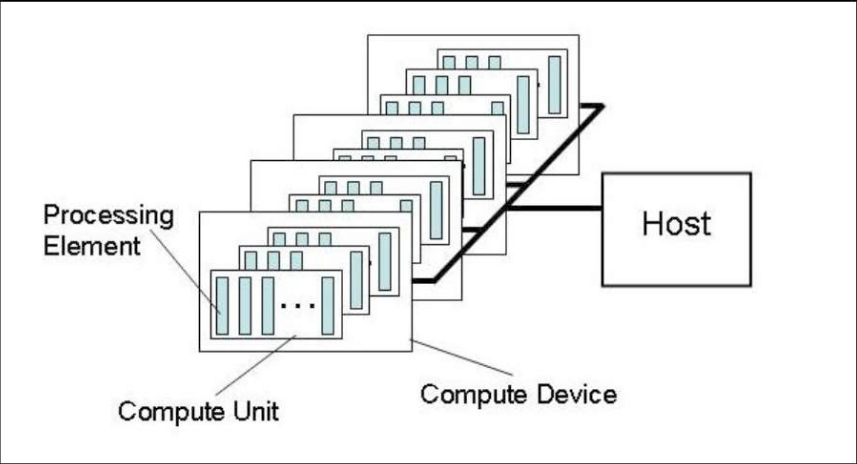
\includegraphics[width=8cm]{images/OpenCLModel.png}
	\caption{An examplary OCT image of the needle}
	\label{ExampleOCTImage}
\end{figure}
\pagebreak
\subsection{Platform}
A core concept of programming with OpenCL is platform. A platform consists of a host and one or more connected devices, in this case OpenCL supports GPUs. A connected device is then further divided into compute units and processing elements. How many processing elements  are grouped into one compute unit varies between vendors and is a relevant factor for the optimization of the OpenCL program. 

An OpenCL application consists of two types of code: host code and device code. The host code is run by a host processor with the objectives of creating a platform, prepare data, transfer data to the device and ultimately send commands to the devices. The device code, also known as kernel code, is the piece of code that will be read and executed by the device only. There is a restriction of device code: it can only be written using C standards, meaning external libraries or methods will not be accepted in kernel code. 

Unlike CUDA, an equivalent implementation of NVIDIA, OpenCL can be used for any device that supports the API. CUDA reportedly has a slightly better performance because it was  designed exclusively for NVIDIA GPU, hence optimized with the architecture, but OpenCL offers more flexibility with a competitive performance. 
\subsection{Memory model}
The OpenCL memory model is composed of three layers, global memory, local memory, work group memory. The difference between those memory types is how accessible they are to a single processing unit. Global memory can be accessed by any processing unit, but is also the slowest of the three. Local memories can be accessed from processing units that are in the same work group. Every processing unit has a certain amount of private memory, which can be accessed by that unit only. From top to bottom of the memory hierarchy, the size of memory available for global, local and private memory reduces hierarchically. A more concrete presentation of the relationship between processing units could be roughly presented as follow, only roughly accurate because of different specifications between AMD and NVIDIA:

\begin{figure}[H]
	\centering
	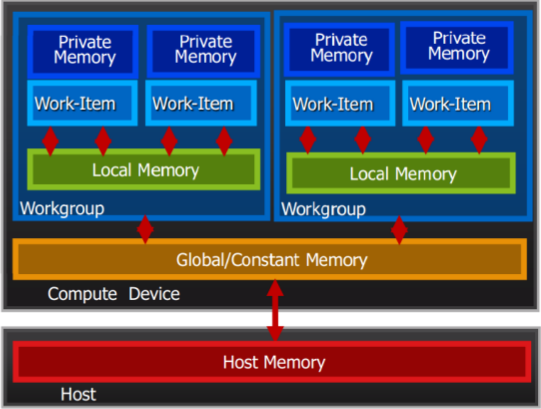
\includegraphics[width=8cm]{images/Model.png}
	\caption{Memory Hierachy}
	\label{ExampleOCTImage}
\end{figure}

\subsection{Execution steps of a OpenCL Program}
OpenCL API allows program to be platform independent, that means it would work with every devices that supports the API. Users can actively manage task, choose device they want to execute the task on and commence execution without deep knowledge of the hardware layer. It does however requires some preparation steps from the host to configure the OpenCL Model. The steps should be carried out in order as following:
\begin{itemize}
	\item Accessing Platform: The step of choosing which platform to execute the kernel code on. OpenCL provides a data structure named cl\_platform\_id and a method clGetPlatformIDs to assist with the issue. Calling clGetPlatformIds with a result array as arguments results into an array of available platform. Users can also define how many platforms they are looking for and the function uses it as a boundary for the search. Furthermore, more detailed information about a certain platform will be presented with the help of function clGetPlatformInfo (Vendors, Version, Profile et cetera).
	\item Accessing Device: Once the Platform has been selected, users can access all the available devices in the machine. A device is represented with cl\_device\_id data structure. Similar to the previous step, a method is provided to enlist all the devices available: clGetDeviceIds. Optimization often requires specification such as work size and the work group number of the device being used. This is where clGetDeviceInfo becomes very useful: it provides all the specification of the selected device.
	\item Creating Context: To add command queue and execute it, a context must be created for the selected platform. The context from a platform can only accept devices from the same platform’s vendor. It means an AMD GPU and an NVIDIA GPU can not run on the same context, there must be two for each of them. Context is represented by cl\_context data structure, which could be created using clCreateContext() or clCreateContextFromType().
	\item Creating Program:  After gathering all the information needed about the hardware, it is time to create the OpenCL Program. A Program is a cl\_program data structures which holds all the kernels together. In order to successfully create a program, a source file or a binary file storing all kernel method is required. Then depending on which kind of source file is being used, clCreateProgramWithSource() or clCreateProgramWithBinary() should be used to create the program. 
	\item Build Program: The created program still needs to be built, or differently speaking to be compiled by OpenCL Compiler, which must be done with clBuildProgram() method. This step could be very troublesome as the compiler expects the source file to contain kernels without syntax errors. In case there is one the build will fail and return -1. To ease up the kernel debugging process there is an option of using clGetProgramBuildInfo() to print out a trace of all possible problems the compiler could find in the kernel code.
	\item Creating Function kernels: Unlike traditional programming practice, methods can not be called directly, but need to be packed in a cl\_kernel data structure first. Every function that will be called needs to be packed in a kernel object and these objects can be reused multiple times. Alternatively an array of kernels could be created and packed by using clCreateKernelsInProgramm(). 
	\item Setting arguments for kernel:  In case there are function arguments, these must be added into newly created kernel objects. Every argument should be packed into a cl\_mem object, which can be created by using clCreateBuffer(). Using this method, programmers have the choice of how the memory should be created and initialized, if it should be read only or read and write, or write only. These options are made available by implemented flags inside the function. Performance differences between those options could be very high for a real time system. The main reason behind the difference is how the memory should be initialized, by default or by user input. In the case of user initialized memory, it takes time to transfer from host to device, which depends on the speed of the computer’s PCI Express. Memory transferring between host and pointer is generally a slow process in proportion to internal memory access speed, hence it is recommended to reduce the amount of memory transferred as much as possible. Another reason for caution in this step is to define the right amount of memory required, because if the size of the memory created is smaller than needed, the program will still function and give back unexpected behavior which could be hard to debug. After creating the cl\_mem buffer object, it is still necessary to tell kernel objects which buffer object belongs to which kernel function and the corresponding index of the arguments in function. OpenCL API provides the function clSetKernelArg() to bind the buffers to the arguments of kernel. The parameters needed for this function are the index of corresponding argument value, size of buffer object and a pointer to the buffer.
	\item Creating Command Queue: The execution of kernel methods must be managed by a command queue. Given the context and program created in previous steps, a new command queue could easily be created by using clCreateCommandQueue(). The method returns a cl\_command\_queue object and its reference count could be retained by clRetainCommandQueue() or decremented with clReleaseCommandQueue(). The queue follows the first-in-first-out principle, meaning a task that was added first into the queue will be executed firstly.
	\item Enqueue Kernel: The purpose of this step is to set the created arguments to the kernel object to an queue and execution.  There are two functions created to accomplish this task: clEnqueueTask() and clEnqueueNDRangeKernel(). The first one, clEnqueueTask, is not frequently used in real world OpenCL application. It only allows to execute kernel within one single work item, which is not the point of parallelism. In fact it was only used in tutorials as introduction to OpenCL. The second one, clEnqueueNDRangeKernel() is more complicated and widely used. Within this function, users can define the dimensions of work groups, local work size, work offset, et cetera. These factors will be explained further in the next chapter about what they are, and why they play an important role in overall performance. After calling this function, the command will be executed in the device. On a further note, if there are severals kernel on the queue and each one of them needs to be executed before moving on to the next, clFlush() and clFinish() should be called right after.
	\item Reading from Buffer Object: After executing kernel, users can read the result from the buffer objects, which could be done by calling clEnqueueReadBuffer(). In this method, the buffer object, a destination array (allocated memory for large arrays to avoid segmentation fault), a size of the memory to be read, and in some case, offset, should be defined. The function returns 0 when executed properly without error.
\end{itemize}

These steps are required to run an OpenCL Application properly. Every method mentioned allows the user to define a variable for storing and debugging error code. As usual, 0 means everything works, other numbers indicate an error. There are various types of error codes, which are also listed by OpenCL specification, of why and where they happen. However, these steps do not need to be repeated every time users want to run another kernel command. Step 1 - 5 are only needed to run once after the program starts as preparation. It should only be run once, because the time needed to compile kernel code from a source could be very slow. In this thesis, when a performance time is mentioned, it is also implied that the preparation steps are not included, because they only need to be executed after the start up. As discussed before, there are some parameters that need to be configured in these steps to improve the performance of the program, but before going into details about those configurations, a good understanding of work group and work items is required, which will be the focus of the next chapter. 

\subsection{Global, local work size, work groups}
The difference the GPU programming makes in comparison to the CPU is the ability of running many more threads at the same time. In the steps described in the previous chapter, there is not yet a defined number of threads to be executed. The first question to be answered before trying to parallelize a program is how many threads are needed. For OpenCL it does not matter how many threads the users want, the program will execute anyway because of its management mechanism. The reason behind this is that if the number is more than the ones that are available, OpenCL will execute those surplus threads as soon as there are threads available again. This, while being very flexible, eliminates the advantage of parallelism.

Secondly, knowing how many work items are available, assuming the device is not preoccupied by graphical task of the computer, is important for designing the program. As mentioned before, OpenCL provides the method clGetDeviceInfo() allowing users to have a closer look into the specification of the device. Furthermore, users can run the command “clinfo” to access the full information about all the platforms available from the terminal, given that OpenCL is installed correctly. The result will be a list of platforms and the devices available in each platform, the specification of these devices with critical information pieces like Vendor, Version, Version of Supported OpenCL, Clock frequency, et cetera. In this chapter, “Max work item dimensions”, “Max work item sizes”, “Max work group size” will be discussed further. The following picture shows an example of the result when clinfo is called:

\begin{figure}[H]
	\centering
	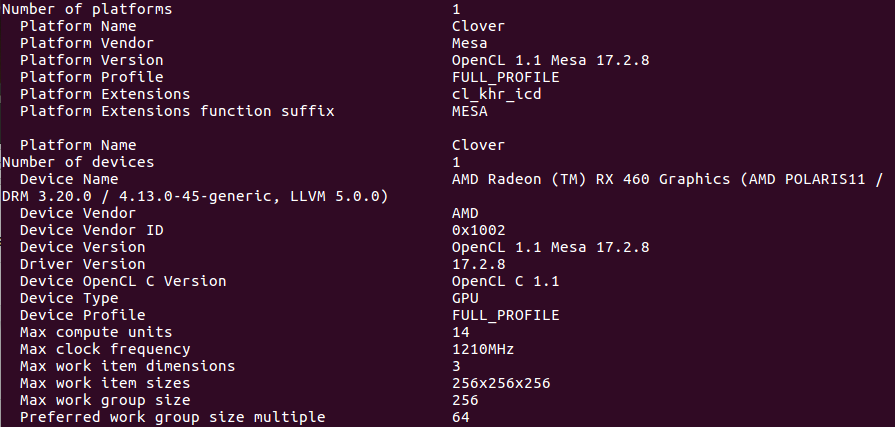
\includegraphics[width=12cm]{images/clinfo.png}
	\caption{Information about current available devices}
	\label{ExampleOCTImage}
\end{figure}

Threads in the GPU programming world can also be called as work items, since work items are meant to be executed parallelly. For the sake of simplicity the device shown in the last picture will be used as an example. In this example it is a low end AMD graphic card and has the max work item size of 256x256x256. The numbers show the max number of work items available in each dimension. It is similar to a 3D coordination system and hence the number of all work items available can be calculated as: 256 x 256 x 256 = 16,777,216 work items. In comparison with off the shelf CPUs, the number of work items of a GPU is far more superior.

In the scope of this thesis, the number of threads available is far more than what is needed (around 1-2 million work items). It is still necessary to inform OpenCL the number of threads the application needs, which leads to the definition of global work size. Global work size is basically  the number of threads a user needs. It does not have a limit, meaning a user can define the global work size as much as they like, as long as the device global memory is not exceeded. The global work size can have as much as three dimensions, but it does not necessary need to. For some special tasks it would be very practical to use more than one, for example image processing with two work size dimensions. But in all cases, using one dimension is intuitive, sufficient and often more advantageous for optimization, which will be explained later. Following is a simplified presentation of work group and work items:

\begin{figure}[H]
	\centering
	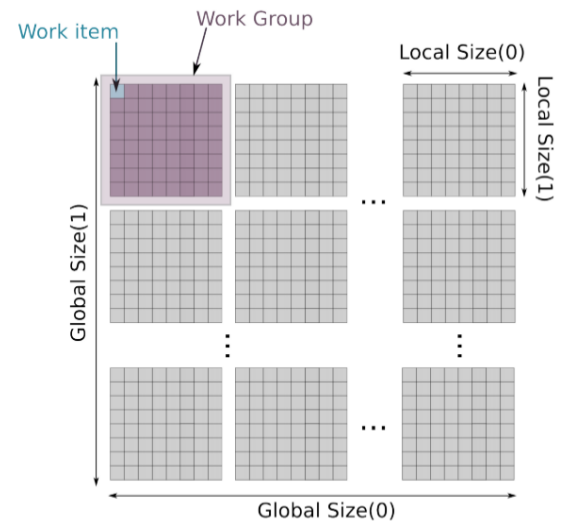
\includegraphics[width=10 cm]{images/itemunit.png}
	\caption{Information about current available devices}
	\label{ExampleOCTImage}
\end{figure}

On the other hand, local work size can not be as arbitrary big as users want, it is constraint by the specification of the device. The limit of the local work size is also defined by the max number of work items per dimension, in the example it is 256 items per work group per dimension. Unlike the global work size, it is not obligatory to define the local work size, users can define it as NULL if they wish to. In this case, OpenCL will handle the local work size itself.

A work group is basically a set of work items that are grouped together. The number of work group can be dynamic, as it depends on the number of the global work size and the local work size. Grouping work items together can have certain positive effects on the performance, since work items in the same work group are synchronized much better and can have access to local memory, which could be advantageous. It is also critical to set the global work size to be a natural multiple of the local work size. For example, if a local work size of 128 is defined, then the global work size must be 128*n where n is a natural number.

Each GPU vendor has developed their own optimization strategy with a prefered local work size definition. As mentioned before, the only constraint between the local and global work size is only that the local work size should be the natural divisor of global work size. Configuring the right local work size has a positive impact to the overall performance. NVIDIA recommends for their GPUs a multiple of 32 for local work size, while for AMD equivalent the recommendation is a multiple of 64. (SOURCE). The reason behind the performance improvement is the architecture of the GPU: A wavefront (fundamental work unit of AMD GPUS) consists of 64 work items, thusly a multiple of 64 local work size will not require a regroup of work-items, therefore provides better performance. The same explanation applies to NVIDIA GPUs.

Global, local work size and work group are very important terminologies in GPU Programming. A good knowledge and correct information of the specification of  the device can boost up the performance quite significantly.
\newpage

\subsection{Kernel}

As explained previously, kernel code is the piece of software that is actually executed in the device. Writing a comprehensive, efficient and error-free kernel code can be quite challenging for programmers without previous low level programming experience. The most important aspects of kernel code is the private memory management, syntax, and utilisation of available memory. One important aspect to be concerned about is that the resource (memory, calculating power) available for one work unit is very limited. This explains why it is very important to reduce the workload in each kernel function as much as possible.

There are several constraints to be concerned about while writing a kernel function. The following code snippet is an illustration for a simple kernel method with OpenCL. The function adds two elements of two arrays and write the result to a third array:
\begin{lstlisting}
__kernel void hello(__global int *a, __global int *b, 
					__global int *c) {
        int gid = get\_global\_id(0);
        C[gid] = a[gid]+b[gid];
    }

\end{lstlisting}

Every kernel function, with an exception of auxiliary functions, must have the identifier “\_\_kernel” and void as return value. Passing parameters consists of three arrays, all of them have “\_\_global” as identifier, indicating the source of the arguments. There are three different kinds of identifiers in the memory model as mentioned before: “\_\_global”, “\_\_local”, “\_\_private”. Note that it is required to pass pointers to the function, regardless what data type it is: an array, an int, float or a customized data structure.

There are some built in options of array representation in OpenCL. For each primitive data type there are severals options to represent an array with that type with a predefined size, for example: float4, int4, char4 et cetera. Users can also use normal array structures used in the C programming language.  As previously discussed, the maximum size of arrays is quite limited due to the lack of memory available. It is recommended to use global or local memory depending on the required array length. Following listing shows an example of TODO

In kernel function, it is impossible to use functions from external libraries. However, the API supports standard C library with its useful arithmetic functions like max, min et cetera. With more complicated functions, for example the correspondence matching function which will be later implemented, it is recommended to divide the function into smaller parts and rewrite it into C conformed functions. It is often the case that a piece of code is quite often reused in kernel, therefore programmers have the possibility to pack it into an auxiliary function, which still follows the principle with identifiers for passing arguments.

The execution model of OpenCL works on the principle that every work item knows what to do and can be independent on the work of other work items. On the very first line of the code, the function get\_global\_id() is called and saved as an index for the elements to be added. The function call returns the unique work item index of the first dimension of work sizes (index starts at 0), since in this sample only one work dimension is used.

One big challenge of writing kernel in OpenCL is the lack of a built in debugger tool or the possibility of  looking to the steps that are being taken. However, there are several external programs that could be helpful for analyzing, profiling the application like CodeXL, GPUVerify from the Imperial College of London or Oclgrind from the University of Bristol. These applications allow users to run kernel with customized arguments, profile execution time, running kernel step by step. However, having a good strategy for parallelizing is the best way to prevent errors in execution.
